\chapter{Prototipo de Exploración}\label{cap.prototipoExploracion}

En este capítulo se describe la creación del primer prototipo del proyecto, el prototipo de exploración, en él se explica la configuración de la placa R-Pi, la conexión de los sensores y el código utilizado para la lectura de los mismos. Por último se realizan algunas pruebas para demostrar el correcto funcionamiento y su rendimiento.


\section{Desarrollo del Sistema}

\subsection{Configuración de la Raspberry-Pi}
En primer lugar, debe instalarse en la placa de desarrollo el sistema operativo que vamos a utilizar, existen varias opciones posibles pero se ha optado por la más habitual denominada Raspbian o Raspberry-Pi OS.
La tarea resulta bastante sencilla simplemente siguiendo los pasos de la página oficial, a través de la cual disponemos de la opción automática de usar un instalador (RaspberryPi Imager) en el que seleccionaremos el lugar de almacenamiento del sistema (la tarjeta Micro SD) y el sistema operativo elegido y únicamente tendremos que esperar a que haga todo el trabajo de escritura. La Figura~\ref{fig:raImager} muestra la interfaz del programa Raspberry Pi Imager.

\begin{figure}[tbh]
\centering
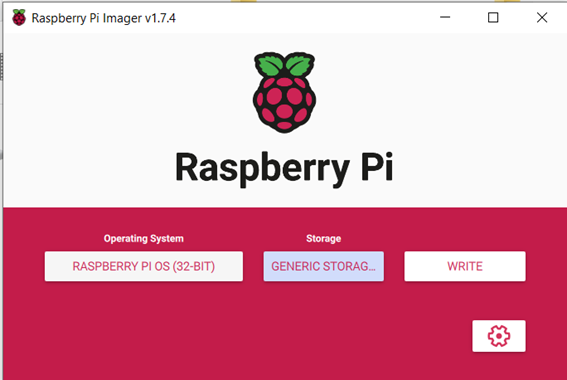
\includegraphics[scale=0.6]{images/raspberryImager}
\caption[Interfaz instalación Raspberry Pi]{Interfaz principal de la aplicación de instalación de sistemas operativos Raspberry Pi: {\protect\tt imager}.}%
\label{fig:raImager}
\end{figure}

Una vez terminado el proceso de instalación, podemos proceder a introducir la tarjeta Micro-SD en la placa R-Pi y realizar todas las conexiones pertinentes para poder arrancar el sistema. Para ello se debe conectar la alimentación, red por cable o posteriormente configurar la WIFI, un teclado, un ratón y un monitor a través de HDMI. 
El proceso es sencillo, seleccionar idioma, zona horaria...etc. Tras unos minutos dispondremos de la placa R-Pi con el sistema operativo plenamente funcional y con una interfaz gráfica muy similar a un Linux.

Tras realizar estos pasos podemos proceder a modificar la contraseña de la placa R-Pi para securizarla a través del menú de configuración o a través de terminal ejecutando el comando\\
\begin{lstlisting}[style=terminal]
sudo raspi-config\end{lstlisting}

Otro punto importante a modificar es en el apartado <<Interface Options>>, es en esta sección a través de la cual debemos activar o desactivar las diferentes opciones de interfaces.\\

En las Figuras \ref{fig:cambioContra} y \ref{fig:interfaceOpt} pueden observarse las opciones de modificación de contraseña y configuración de interfaces comentadas anteriormente.

\begin{figure}[tbh]
\centering
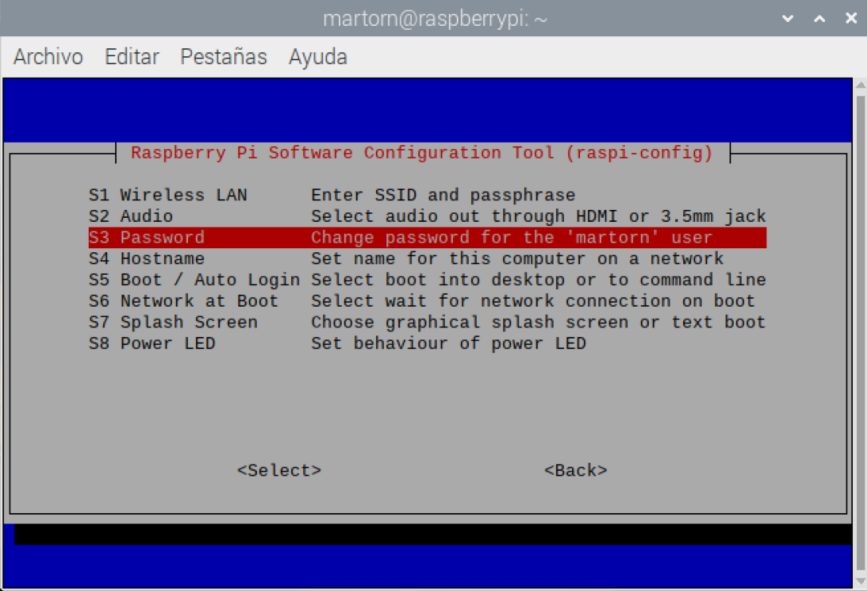
\includegraphics[scale=0.7]{images/raspiConfigPass}
\caption[Cambio de contraseña de Raspberry Pi]{Menú de configuración inicial para realizar el cambio de contraseña: {\protect\tt Password}.}%
\label{fig:cambioContra}
\end{figure}

\begin{figure}[tbh]
\centering
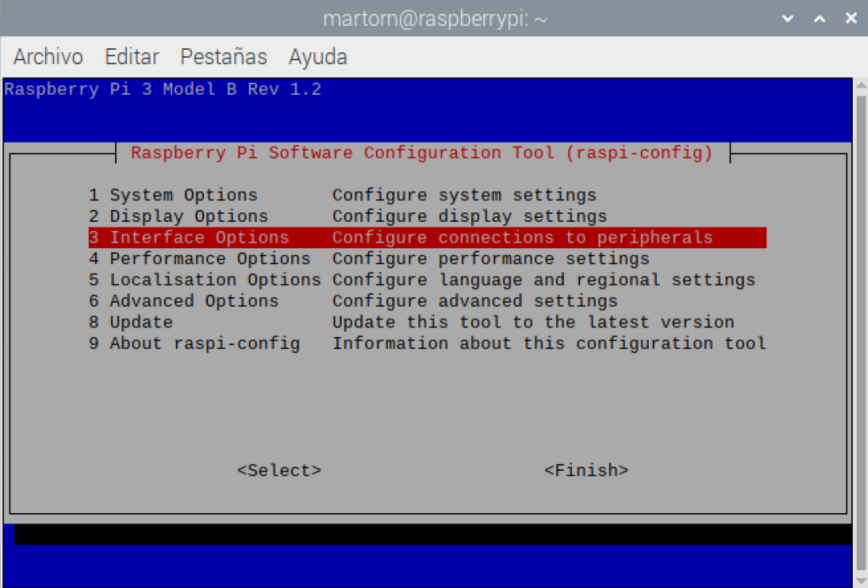
\includegraphics[scale=0.7]{images/raspiConfigInterface}
\caption[Configuración de interfaz de Raspberry-Pi]{Menú de configuración inicial para configuración de interfaces: {\protect\tt Interface Options}.}%
\label{fig:interfaceOpt}
\end{figure}

En la configuración de interfaces activaremos: \textbf{SSH, VNC, SPI, I2C, Serial y Remote GPIO.}

En primer lugar, SSH y VNC permitirán contactar de manera remota con la placa R-Pi para poder acceder a ella o programar, por otro lado, SPI e I2C serán los protocolos de conexión con los sensores que utilizaremos, por ello es importante que estén activos, las otras dos opciones darán acceso a otras funcionalidades de la placa.

\section{Conexión con Raspberry-Pi}
\subsection{VNC Viewer}

Una de las opciones más sencillas para trabajar cómodamente con la placa R-Pi, evitar tantas conexiones y el uso de un monitor externo, es el uso de la herramienta VNC Viewer, con ella se podrá visualizar directamente el entorno gráfico de la placa R-Pi exactamente igual que si estuviéramos conectados por HDMI, en el caso de usar SSH no dispondríamos de entorno visual, es por ello que esta herramienta resultará muy útil.

Para poder utilizar VNC Viewer se debe descargar de la página oficial el instalador y seguir los pasos de instalación, una vez instalada únicamente se debe configurar la conexión con la placa R-Pi determinando la dirección IP de la misma con su respectivo usuario y contraseña como se observa en la Figura~\ref{fig:VNC} para así poder acceder. Tras realizar estos pasos dispondremos de la interfaz gráfica plenamente operativa desde nuestro PC.

En resumen, con esta herramienta obtenemos el beneficio de disponer de la interfaz gráfica totalmente funcional desde nuestro PC como si de una máquina virtual se tratara y a su vez nos evitamos la conexión del teclado, el ratón y el monitor por HDMI a la placa R-Pi.

\begin{figure}[tbh]
\centering
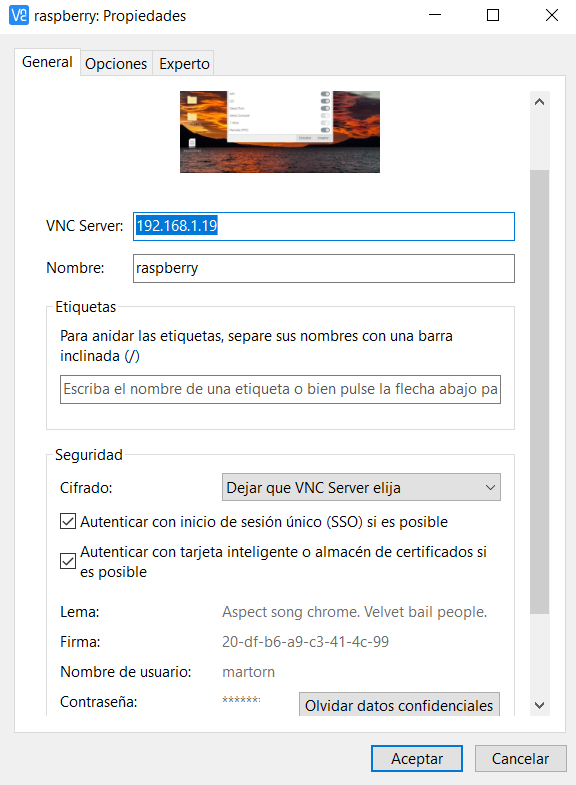
\includegraphics[scale=0.8]{images/vnc.png}
\caption[Configuración de VNC Viewer]{Pestaña propiedades de la aplicación VNC Viewer: Configuración de ejemplo para la conexión con la placa R-Pi.}%
\label{fig:VNC}
\end{figure}

\subsection{Conexión USB to Serial Port}
Otra de las opciones para realizar la comunicación con la placa de desarrollo es la utilización de un adaptador USB a Serial, en concreto un dispositivo FTDI232, mostrado en la Figura~\ref{fig:serial}.

\begin{figure}[tbh]
\centering
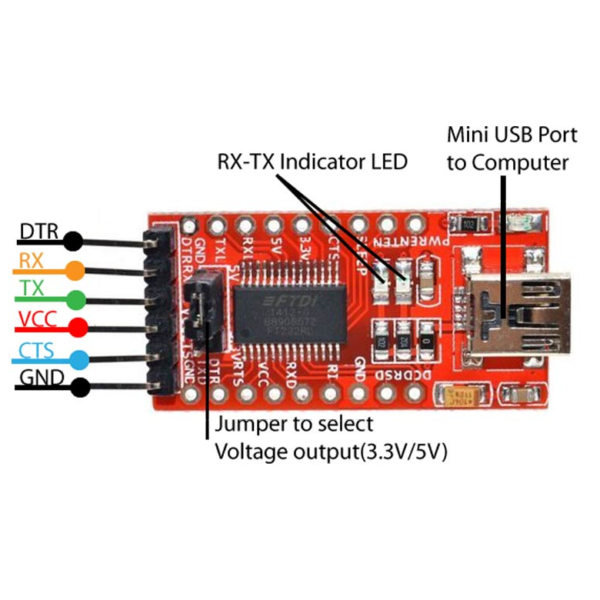
\includegraphics[scale=0.5]{images/serial.png}
\caption[Descripción pines para FTDI232]{Imagen con descripción de los pines del dispositivo para conexión Serial-FTDI232.}%
\label{fig:serial}
\end{figure}

Este dispositivo permite el envío de información directamente al puerto USB del dispositivo al que lo conectemos, en este caso un PC. Para que funcione debe realizarse la conexión de tres de sus pines; Rx, Rt y GND, la alimentación la recoge del puerto USB. Estos pines deben conectarse a la placa R-Pi al contrario; Rx a Rt y viceversa. Rx y Rt son los pines 14 y 15 de la placa R-Pi como puede observarse en la Figura~\ref{fig:Rxrt} figura. 

\begin{figure}[tbh]
\centering
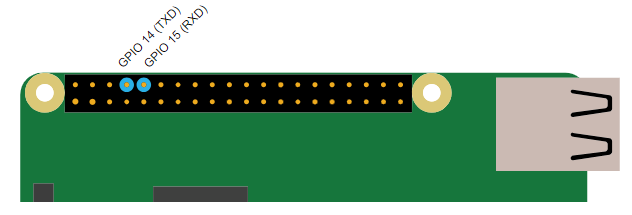
\includegraphics[scale=0.7]{images/serialRasp.png}
\caption[Configuración RX y RT en Raspberry Pi 3]{Localización de los pines RX y RT en el modelo de Raspberry-Pi 3.}%
\label{fig:Rxrt}
\end{figure}

En la placa R-Pi debe activarse la opción de conexión serial que vimos en el apartado de configuración de la Raspberry-Pi, en este caso ya se encuentra activada.

Una vez realizada la conexión, debemos revisar el administrador de dispositivos de nuestro PC para encontrar dónde se ha conectado el dispositivo, en nuestro caso se trata de COM7 (Figura ~\ref{fig:com7}), una vez conocida la linea serie ya podemos configurar el programa Putty para que lea en esa dirección (Figura~\ref{fig:puttyConf}) y por tanto podamos acceder a la placa R-Pi.

\begin{figure}[tbh]
\centering
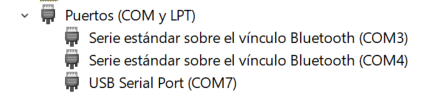
\includegraphics[scale=1]{images/serialCOM.png}
\caption[Puertos COM y LPT en Windows]{Captura de lista de puertos COM y LPT en el administrador de dispositivos de Windows, puede observarse USB Serial Port como COM7.}%
\label{fig:com7}
\end{figure}

\begin{figure}[tbh]
\centering
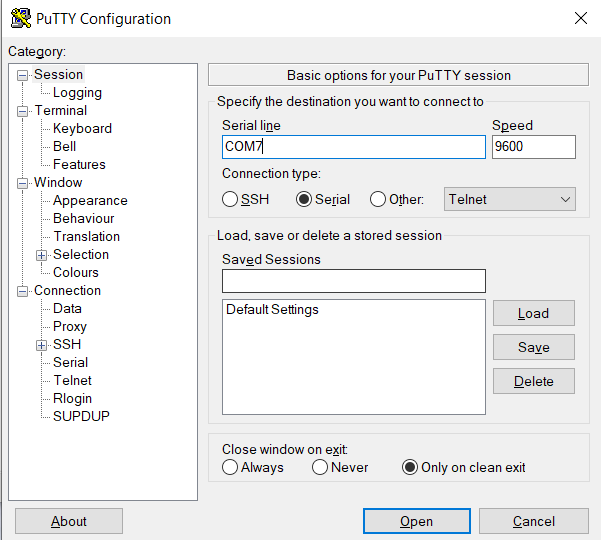
\includegraphics[scale=0.8]{images/putty.png}
\caption[Configuración de Putty para conexión con Raspberry-Pi]{Configuración de la herramienta Putty en Windows para realizar la conexión con la placa R-Pi a través del puerto serie ({\protect\em Serial Port}).}%
\label{fig:puttyConf}
\end{figure}

Al lanzar Putty obtenemos la salida deseada, la placa R-Pi solicita el inicio de sesión mediante usuario y contraseña y, en este momento ya podemos hacer pleno uso de la misma como si estuviéramos en su terminal, en la Figura~\ref{fig:puttyOK} se muestra su visualización:

\begin{figure}[tbh]
\centering
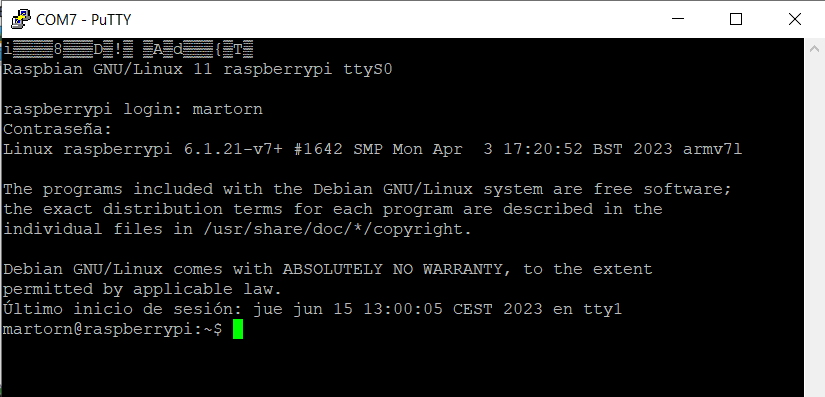
\includegraphics[scale=0.9]{images/puttyOK.png}
\caption[Primer acceso de Putty a Raspberry-Pi]{Visualización del primer acceso desde el terminal de Putty a la placa R-Pi a través de Serial Port.}%
\label{fig:puttyOK}
\end{figure}


\section{Conexión y configuración de los sensores}

Para afrontar el problema se plantean las posibles opciones disponibles, el primer paso es realizar una búsqueda de información sobre el sensor que se desea utilizar, sobre como conectarlo a la placa R-Pi y sobre el lenguaje a utilizar.

En cuanto a las opciones sobre protocolos existen dos: I2C y SPI, para este tipo de proyectos se usa de manera más habitual I2C ya que no se mueve gran densidad de datos y requiere de menos conexiones que SPI, igualmente se barajan ambas posibilidades, es por ello que veremos sus ventajas y desventajas y valoraremos cuál es la mejor opción para este tipo de proyecto. A continuación, se presentan algunos puntos a considerar:

\textbf{Número de dispositivos:} Si es necesario conectar múltiples dispositivos a un bus de comunicación, I2C generalmente es más adecuado. I2C utiliza solo dos líneas de comunicación (SCL y SDA), lo que permite conectar varios dispositivos en el mismo bus utilizando direcciones únicas. Al contrario, SPI requiere una línea separada para cada dispositivo conectado, lo que puede limitar la cantidad de dispositivos que se pueden conectar directamente.

\textbf{Velocidad de transferencia:} SPI tiende a tener una velocidad de transferencia más rápida que I2C. En SPI, la velocidad de transferencia se puede ajustar para adaptarse a los requisitos específicos, mientras que I2C tiene una velocidad máxima establecida.

\textbf{Complejidad y pines requeridos:} I2C generalmente requiere menos pines que SPI. Como se mencionó anteriormente, I2C utiliza sólo dos líneas de comunicación, mientras que SPI requiere al menos cuatro líneas (MISO, MOSI, SCK y SS). Si se trabaja con recursos limitados en términos de pines de conexión o es un requisito utilizar la mínima complejidad de cableado, I2C puede ser una mejor opción.

\textbf{Tolerancia al ruido:} I2C tiende a ser más tolerante al ruido que SPI. El protocolo I2C utiliza una topología de bus abierto con drenaje abierto, lo que proporciona una mayor inmunidad al ruido eléctrico. Por otro lado, SPI utiliza señales más nítidas y puede ser más susceptible a interferencias electromagnéticas. Si se trabaja en un entorno ruidoso o con señales propensas a interferencias, I2C podría ser más adecuado.

Por otro lado, en cuanto a los posibles lenguajes de programación a utilizar se han barajado tres posibilidades: Erlang, C y Python. Se harán pruebas con cada uno de ellos para valorar cuál es la mejor opción ya que el objetivo es que se realice una lectura rápida de los datos y de la manera más eficiente.
En estos casos es importante conocer o descubrir la existencia de módulos o librerías ya existentes que nos ofrezcan soluciones más rápidas y sencillas que podamos utilizar para nuestros prototipos.

\subsection{Configuración sensor HMC5983}

El primer prototipo se creará utilizando un sensor HMC5983 y realizando la conexión a través del protocolo I2C, las características de este sensor estarán descritas en la sección correspondiente al mismo. 
Partiendo de la base inicial, el primer paso será realizar las conexiones del sensor a los pines de la placa R-Pi, para utilizar este protocolo necesitamos conectar cuatro de los pines del sensor; VCC (positivo), GND (negativo), SCL y SDA (transmisión de datos). Estos pines serán conectados a la placa R-Pi como se indica en la Figura~\ref{fig:5983Rasp}.

\begin{figure}[th]
\centering
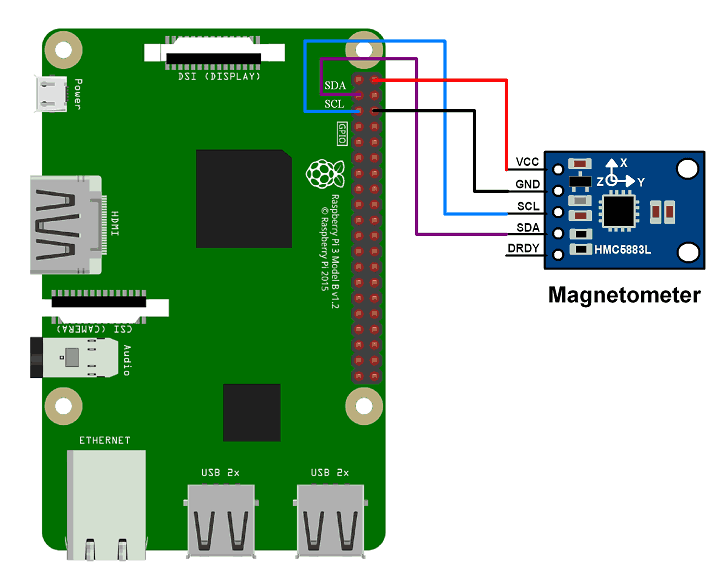
\includegraphics[scale=0.5]{images/conexionRaspHMC5983}
\caption[Conexión HMC5983 a Raspberry-Pi]{Diagrama de conexiones del sensor HMC5983 a Raspberry-Pi 3.}%
\label{fig:5983Rasp}
\end{figure}

Para comprobar que las conexiones se han realizado correctamente, en primer lugar se debe activar el protocolo I2C de la placa R-Pi entrando en su configuración, para ello ejecutamos el comando 
\begin{lstlisting}[style=terminal]
raspi-config
\end{lstlisting}
posteriormente, accedemos a la configuración de interfaces y activamos I2C (enable), tras la realización de estos pasos la placa R-Pi está preparada para recibir datos utilizando este protocolo.Por último, es necesario saber si hemos conectado correctamente el sensor, para ello se ejecuta el comando 

\begin{lstlisting}[style=terminal]
i2cdetect -y 1
\end{lstlisting}
 y se nos mostrará una tabla en la que, en caso de estar todo bien conectado, aparecerá un registro activo como se muestra en la Figura~\ref{fig:i2cDetect}. Podemos observar que se trata de la dirección 0x1E por lo que será aquí donde deberá direccionarse la recogida de datos del sensor
\begin{figure}[th]
\centering
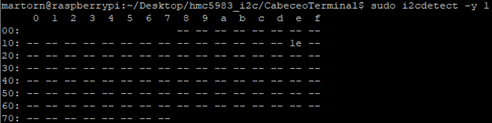
\includegraphics{images/i2cdetect.png}
\caption[Comando <<i2cdetect>> con sensor HMC5983]{Salida del comando <<i2cdetect>> en el terminal de la placa R-Pi tras la conexión con el sensor HMC5983.}%
\label{fig:i2cDetect}
\end{figure}


\subsubsection{Código Python Sensor HMC5983}

El código de este sensor en Python resulta bastante sencillo de encontrar en multitud de páginas web, incluso en la oficial del propio sensor, gracias a esto podemos utilizar códigos ya existentes para adaptarlos a nuestras necesidades lo que ahorra gran cantidad de tiempo. La placa R-Pi no dispone de Python por lo que debe instalarse siguiendo las metodologías habituales, una vez instalado puede pasarse a probar si el código creado lee correctamente nuestro sensor magnetómetro HMC5983. 

El código es sencillo pero consta de varias partes importantes que han de tenerse en cuenta para la posterior programación en otros lenguajes, es por ello que se adjunta el código completo Python que devuelve el cálculo del cabeceo del sensor por terminal para poder así explicar cada una de ellas.

En la primera sección, aparte de importar los módulos necesarios se crean las variables que serán usadas como direcciones de los registros, estas son direcciones representadas como un número hexadecimal obtenidas del datasheet del sensor. El siguiente paso es inicializar el sensor, para ello se establecen ciertos valores en los registros de configuración que establecen el modo y la ganancia del sensor.

La función $read\_raw\_data()$, se utiliza, como su nombre indica, para leer los datos sin procesar, toma la dirección del registro como argumento y lee dos bytes de datos (uno alto y uno bajo), posteriormente, combina los dos bytes en un valor de 16 bits y ajusta el signo en caso de ser necesario.

Tras la realización de estos pasos, se lanza la función que inicializa el sensor para que este empiece a leer de manera continuada, esta función obtiene los datos de los ejes X, Y y Z pero estos aún están sin procesar, es por ello que se calcula el cabeceo utilizando la función \textit{math.atan2()} que devuelve el ángulo en radiantes y por último se suma la declinación al ángulo calculado. Por último, se comprueba si el ángulo es mayor que 2$\pi$ o si es negativo para ajustarlo en caso de ser necesario.\\

\lstset{language=Python, breaklines=true, basicstyle=\footnotesize}
\begin{lstlisting}[frame=single]

import smbus #import SMBus module of I2C
from time import sleep  #import sleep, used for reading frequency
import math

Register_A     = 0              #Address of Configuration register A
Register_B     = 0x01           #Address of configuration register B
Register_mode  = 0x02           #Address of mode register

X_axis_H    = 0x03              #Address of X-axis MSB data register
Z_axis_H    = 0x05              #Address of Z-axis MSB data register
Y_axis_H    = 0x07              #Address of Y-axis MSB data register
declination = -0.00669          #define declination angle of location where measurement going to be done
pi          = 3.14159265359     #define pi value

def Magnetometer_Init():
        #write to Configuration Register A
        bus.write_byte_data(Device_Address, Register_A, 0x70)

        #Write to Configuration Register B for gain
        bus.write_byte_data(Device_Address, Register_B, 0xa0)

        #Write to mode Register for selecting mode
        bus.write_byte_data(Device_Address, Register_mode, 0)
	
def read_raw_data(addr):
    
        #Read raw 16-bit value
        high = bus.read_byte_data(Device_Address, addr)
        low = bus.read_byte_data(Device_Address, addr+1)

        #concatenate higher and lower value
        value = ((high << 8) | low)

        #to get signed value from module
        if(value > 32768):
            value = value - 65536
        return value


bus = smbus.SMBus(1) 	
Device_Address = 0x1e   # HMC5983 Address

Magnetometer_Init()     # initialize HMC5883L magnetometer 

print (" Reading Heading Angle")

while True:
   
        #Read Accelerometer raw value
        x = read_raw_data(X_axis_H)
        z = read_raw_data(Z_axis_H)
        y = read_raw_data(Y_axis_H)

        heading = math.atan2(y, x) + declination
        
        #Due to declination check for >360 degree
        if(heading > 2*pi):
                heading = heading - 2*pi

        #check for sign
        if(heading < 0):
                heading = heading + 2*pi

        #convert into angle
        heading_angle = int(heading * 180/pi)

        print ("Heading Angle = %d" %heading_angle)
        sleep(0.5)

\end{lstlisting}


En la salida obtenida del sensor observada en la Figura~\ref{fig:salidaHMCP}, se puede ver que es correcta y los ángulos se obtienen en bucle hasta finalizar la ejecución del programa de manera manual, a mayores, la frecuencia de lectura es modificable cambiando el valor de sleep() medido en segundos, en este caso 0.5. 

\begin{figure}[th]
\centering
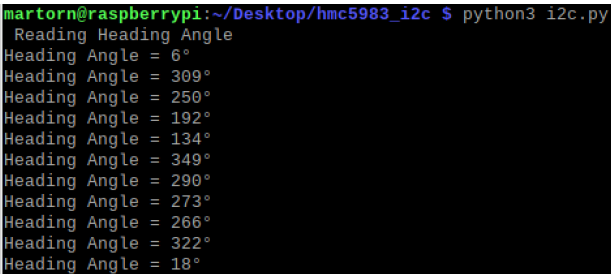
\includegraphics{images/salidaHMC5983Python.png}
\caption[Salida código Python sensor HMC5983]{Visualización de la salida en terminal tras la ejecución del código del sensor HMC5983 implementado en Python.}%
\label{fig:salidaHMCP}
\end{figure}

\subsubsection{Código C Sensor HMC5983}

El código C se ha creado a semejanza del código Python visto anteriormente, a diferencia del anterior, este dispone de la posibilidad de pasarle dos argumentos, el tiempo durante el cual queremos que se lean datos y la frecuencia de lectura de los mismos; a mayores, este programa almacena los datos de cabeceo en un archivo externo que será utilizado para su visualización en el servidor.

Se han encontrado más dificultades para encontrar información sobre este código en este lenguaje, se ha observado que la utilización de Python para la programación de este tipo de sensores es mucho más frecuente. Un punto positivo es que al disponer con anterioridad del programa Python se ha podido utilizar como base. La mayor diferencia y el gran beneficio de la utilización del lenguaje C en el caso de este proyecto es la compatibilidad que tiene con Erlang, esto será una gran ventaja de cara a la programación del servidor ya que debe comunicarse con el programa que ejecuta los sensores desde la placa R-Pi.

El funcionamiento del código es similar, se inicializa el sensor y se calcula el cabeceo con los datos obtenidos de los ejes X, Y y Z, como se comentó anteriormente. En este código se han añadido algunas mejoras con respecto al anterior: en primer lugar, se permite la introducción de dos argumentos: el tiempo y la frecuencia y en segundo lugar, se crea el archivo en el que se escribirán los datos obtenidos del sensor. El siguiente paso es crear una función que compruebe si el tiempo introducido en el argumento es mayor que el tiempo transcurrido, de esta manera puede conseguirse que el programa termine en caso de llegar al límite de tiempo. Por último se introduce el parámetro de la frecuencia en la variable del $time\_sleep$s.\\

A la hora de compilar el código C, antes de ejecutarlo, es importante enlazar las bibliotecas \textit{pigpio} (Controladora de pines GPIO) y \textit{libm} (funciones matemáticas adicionales), para ello se debe ejecutar el comando de compilación gcc añadiendo -lpigpio -lm como sigue:\\
\begin{lstlisting}[style=terminal]
gcc -o nombreEjecutable nombrePrograma.c -lpigpio -lm
\end{lstlisting}

\lstset{language=C, breaklines=true, basicstyle=\footnotesize}
\begin{lstlisting}[frame=single]
//Importacion de librerias necesarias
#include <stdio.h>
#include <stdlib.h>
#include <pigpio.h>
#include <math.h> 

//Definicion de los registros a utilizar.
//la direccion se ha obtenido ejecutando el comando i2cdetect -y 1 sobre la linea de comandos.
#define HMC5983_ADDR 0x1E 
#define HMC5983_REG_X_MSB 0x03
#define HMC5983_REG_Y_MSB 0x07
#define HMC5983_REG_Z_MSB 0x05
#define PI 3.14159265358979323846

int main(int argc, char *argv[])
{
    if(argc !=3){
        printf("Uso:sudo %s [tiempo_lectura] [ratio_lectura]\n", argv[0]);
        return 1;
    }
    
    double tiempo = atof(argv[1]);
    double ratio = atof(argv[2]);
    
    if (gpioInitialise() < 0) {
        printf("Error al inicializar la biblioteca pigpio\n");
        return 1;
    }

    int handle = i2cOpen(1, HMC5983_ADDR, 0);
    if (handle < 0) {
        printf("Error al configurar el dispositivo I2C.\n");
        return 1;
    }
   
    i2cWriteByte(handle, 0x00); //Configuracion del modo continuo
   

//Creacion del archivo en el que se escribiran los datos
    FILE *fp;
    fp = fopen("/home/martorn/Desktop/hello_erlang/src/sensorData/angulosCabeceo.txt", "w"); // Modo escritura
    if (fp == NULL) {
        printf("Error al abrir el archivo para escritura.\n");
        return 1;
    }

    time_t start_time = time(NULL); // Obtener el tiempo de inicio, utilizado para escribir datos durante el tiempo deseado
    time_t current_time;
    
    printf("Recogida de datos en curso");
    int cont=0;
    while (1) {
        // Lectura de los datos de los ejes x, y y z
        uint16_t x_msb = i2cReadWordData(handle, HMC5983_REG_X_MSB);
        uint16_t x_lsb = i2cReadWordData(handle, HMC5983_REG_X_MSB + 1);
        uint16_t x = (x_msb << 8) | x_lsb;

        uint16_t y_msb = i2cReadWordData(handle, HMC5983_REG_Y_MSB);
        uint16_t y_lsb = i2cReadWordData(handle, HMC5983_REG_Y_MSB + 1);
        uint16_t y = (y_msb << 8) | y_lsb;

        uint16_t z_msb = i2cReadWordData(handle, HMC5983_REG_Z_MSB);
        uint16_t z_lsb = i2cReadWordData(handle, HMC5983_REG_Z_MSB + 1);
        uint16_t z = (z_msb << 8) | z_lsb;

        // Calculo del angulo de cabeceo
        float pitch = atan2((float)x, sqrt(pow((float)y, 2) + pow((float)z, 2))) * 180 / PI;

        // Escritura de los datos en el archivo
        fprintf(fp,"%.2f \n",pitch);
        
        // Obtener el tiempo actual y comprobar si ha pasado el periodo de tiempo determinado de lectura de datos
        current_time = time(NULL);
        if (current_time - start_time >= tiempo) {
            break; // Salir del bucle despues de escribir durante el periodo de tiempo determinado
        }
		// FRECUENCIA DE LECTURA
        for (int i=0; i<cont %4; i++){
            printf(".");
            }
        fflush(stdout);
        cont++;
        time_sleep(ratio); // Velocidad de lectura de los datos, periodo entre lectura y lectura. 
    }
    printf("MagOK");
    i2cClose(handle); //Se cierra la lectura del sensor
    fclose(fp); // Cerrar el archivo
      return 0;
}
\end{lstlisting}

En la Figura~\ref{fig:salidaHMCC} se muestra una salida de ejemplo almacenada en un archivo al ejecutar el programa, en ella observamos una lista de los grados obtenidos durante el tiempo de ejecución separados por un salto de linea.

\begin{figure}[h]
\centering
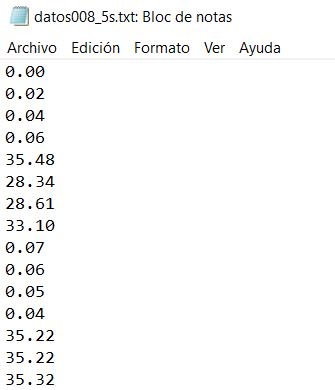
\includegraphics[scale=0.75]{images/salidaHMC5983C.png}
\caption [Archivo de salida código C del sensor HMC5983]{Archivo de salida creado por el código programado en C que lanza el sensor HMC5983}%
\label{fig:salidaHMCC}
\end{figure}


\subsection{Configuración sensor HC-SR04}

El segundo prototipo se creará utilizando un sensor ultrasónico HC-SR04, las características de este sensor están descritas en la sección correspondiente al mismo. 

Partiendo de la base inicial, el primer paso será realizar las conexiones del sensor a los pines GPIO de la placa R-Pi, para crear este enlace necesitamos conectar los cuatro de los pines del sensor; vcc (positivo), GND (negativo), echo (receptor de señales) y Trig (transmisor de señales). Estos pines serán conectados a la placa R-Pi de la siguiente manera:
\begin{itemize}
    \item \textbf{VCC}: 5V - PIN 2
    \item \textbf{GNC}: Negativo - PIN 6
    \item \textbf{Trig}: GPIO 17 - PIN 11
    \item \textbf{Echo}: GPIO 27 - PIN 13
\end{itemize}
Como puede observarse en el diagrama de conexiones de la Figura~\ref{fig:diagramaConexionesHC}, la conexión del sensor tiene la peculiaridad de necesitar usar dos resistencias: una de 330 \(\Omega\) y otra de 470 \(\Omega\), esto se debe a que los pines GPIO toleran un máximo de 3.3V y el sensor debe conectarse a 5V. En nuestro caso utilizaremos de manera similar dos resistencias: una de 1k\(\Omega\) y otra de 2.2k\(\Omega\)


\begin{figure}[h]
\centering
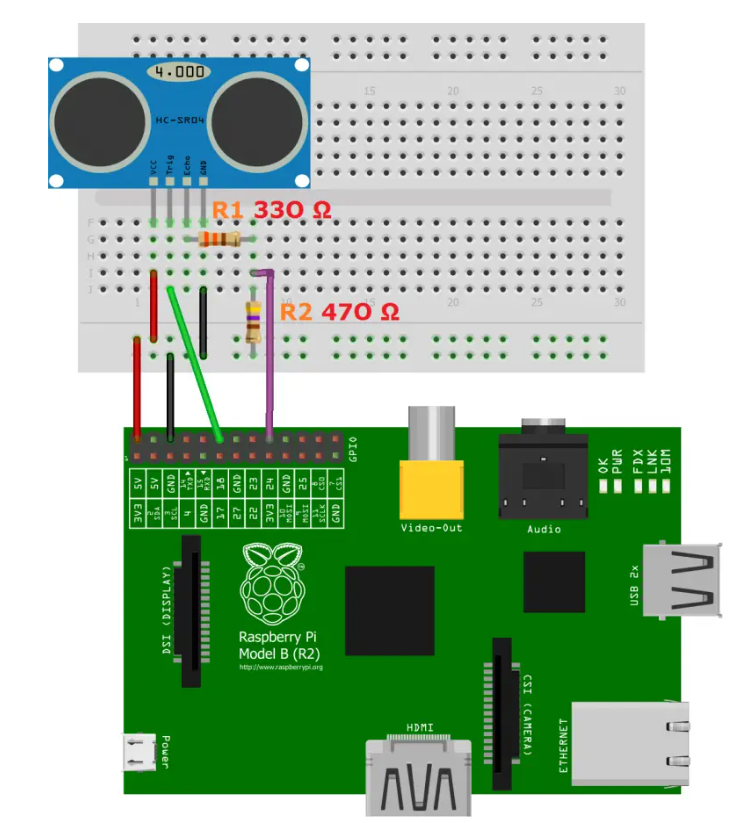
\includegraphics[scale=0.65]{images/conexionRaspHCSR04.png}
\caption[Conexión HC-SR04 a Raspbery-Pi]{Diagrama de conexiones del sensor HC-SR04 a raspberry-Pi 3.}%
\label{fig:diagramaConexionesHC}
\end{figure}

Una vez creada la conexión, se puede comenzar a crear el código que recibirá los datos del sensor. 

\newpage
\subsubsection{Código Python sensor HC-SR04}

El código Python de este sensor resulta bastante sencillo de implementar debido a la amplia cantidad de información que se encuentra al respecto en diversas páginas o manuales, a continuación se explican las partes más importantes del mismo. 

En el caso de Python utilizaremos la biblioteca RPi.GPIO que proporciona acceso directo a los pines GPIO de la placa R-Pi. Gracias a esta biblioteca podemos determinar el modo de numeración de los pines, en este caso que se establece como BCM(Broadcom SOC chanel) utilizando \textit{GPIO.setmode} y \textit{GPIO.setup}, esto nos permite determinar cuál es el pin de entrada (Echo (GPIO 27)) y cuál el de salida (Trig (GPIO17)).

El siguiente paso es crear la función que mide la distancia, esta establece el pin Trig en alto durante un corto periodo de tiempo para activar el pulso de disparo de ultrasonido del sensor y luego se espera un breve tiempo antes de establecer el mismo pin en bajo para finalizar el pulso. Registrando los tiempos de inicio y fin del pulso (pulse\_start y pulse\_end) se puede medir la duración del pulso ultrasónico reflejado, para ello se entra en un bucle mientras el pin ECHO esté en estado bajo, lo que indica que aún no se ha recibido el pulso ultrasónico reflejado. Durante este tiempo, se actualiza continuamente el valor de $pulse\_start$ con el tiempo actual hasta que se detecte el inicio del pulso reflejado.Después, se entra en otro bucle mientras el pin ECHO esté en estado alto, lo que indica que el pulso ultrasónico reflejado está siendo recibido. Se actualiza constantemente el valor de $pulse\_end$ con el tiempo actual hasta que se detecte el final del pulso reflejado.

Por último, se realiza el cálculo de la distancia utilizando el inicio y fin del pulso obtenido anteriormente. Este cálculo se basa en dividir la duración del puso entre dos y multiplicarlo por la velocidad del sonido del aire (aproximadamente 34000 cm/s). La distancia se calcula como la mitad del tiempo total de ida y vuelta del pulso, ya que el pulso viaja desde el sensor hasta el objeto y vuelve al sensor.

A través de este código obtenemos por terminal un bucle de datos de distancia, medida en centímetros, con un ratio que puede ser modificable estableciendo diferentes valores en el $time.sleep()$ del <<try>>. En la Figura~\ref{fig:salidaUltrasonidoP} se puede observar una salida de ejemplo. 

\begin{figure}[h]
\centering
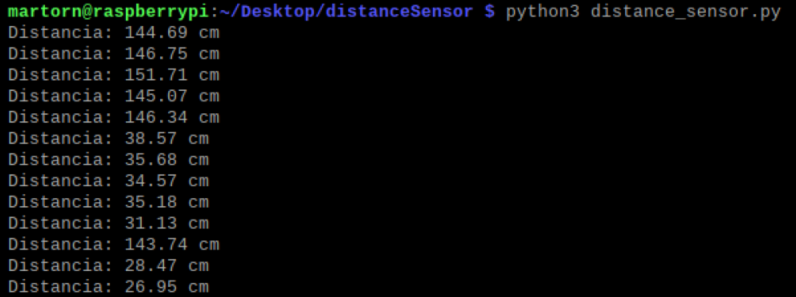
\includegraphics[scale=0.8]{images/salidaUltrasonidoPython.png}
\caption[Salida terminal del código Python del sensor HC-SR04]{Visualización de la salida del terminal de la placa R-Pi del código programado en Python que lanza el sensor HC-SR04.}%
\label{fig:salidaUltrasonidoP}
\end{figure}

\lstset{language=Python, breaklines=true, basicstyle=\footnotesize}
\begin{lstlisting}[frame=single]
import RPi.GPIO as GPIO
import time

GPIO.setmode(GPIO.BCM)

TRIG_PIN = 17
ECHO_PIN = 27

GPIO.setup(TRIG_PIN, GPIO.OUT)
GPIO.setup(ECHO_PIN, GPIO.IN)

def measure_distance():
    GPIO.output(TRIG_PIN, True)
    time.sleep(0.00001)
    GPIO.output(TRIG_PIN, False)

    pulse_start = time.time()
    pulse_end = time.time()
    
    while GPIO.input(ECHO_PIN) == 0:
        pulse_start = time.time()

    while GPIO.input(ECHO_PIN) == 1:
        pulse_end = time.time()

    pulse_duration = pulse_end - pulse_start
    distance = pulse_duration * 34300 / 2

    return round(distance, 2)  # Redondear la distancia a 2 decimales

try:
    while True:
        dist = measure_distance()
        print("Distancia:", dist, "cm")
        time.sleep(0.5)

except KeyboardInterrupt:
    print("Programa interrumpido por el usuario")

finally:
    GPIO.cleanup()
\end{lstlisting}

\subsubsection{Código C del sensor HC-SR04}

El código C utilizado para la lectura de distancia del sensor ultrasónico se ha basado en el funcionamiento del código Python ya que la lectura de este tipo de sensores no suele implementarse en este lenguaje. A diferencia del código anterior, la biblioteca principal utilizada para acceder a los pines GPIO será \textit{wiringPi}. Otra diferencia es que en este código se ha implementado la funcionalidad de poder modificar el tiempo y el ratio de lectura, y además los datos serán guardados en un archivo de texto para que puedan ser visualizados desde el servidor.

La manera de implementar la lectura es similar al código Python. En primer lugar, es importante definir qué pines representarán TRIG y ECHO para posteriormente configurar TRIG como salida y ECHO como entrada mediante el comando \textit{wiringPiSetupGpio()}. El siguiente paso es, al igual que en el código Python, activar el pulso de disparo enviando un pulso corto al pin TRIG, medir el <<tiempo de vuelo>> del pulso (tiempo entre activación y recepción del eco) y realizar el cálculo pertinente para convertir el tiempo en distancia.

Además, en este código se introduce la posibilidad de que el eco del pulso no se detecte o este sea demasiado largo para que esos valores no sean almacenados ya que no son útiles.

Por último, nos encontramos con la función principal \textit{main()}, que se ocupa de que lo siguiente:
\begin{itemize}
    \item  Verificar que los argumentos necesarios sean introducidos correctamente, en este caso dos: el tiempo de lectura y el ratio de lectura.
    \item Llamar a la función que configura los pines GPIO, denominada \textit{setup()}.
    \item Abrir un archivo en modo lectura en el que se escribirán los datos obtenidos por el sensor
    \item Crear un bucle de recogida de datos que se ejecute hasta que se alcance el tiempo especificado por el argumento introducido anteriormente. En cada iteración se llama a la función que obtiene la distancia y se almacena el dato obtenido en el archivo abierto.
    \item Controlar la frecuencia de lectura de datos utilizando \textit{time\_sleep()} con el argumento introducido.
\end{itemize}
\clearpage

\lstset{language=C, breaklines=true, basicstyle=\footnotesize}
\begin{lstlisting}[frame=single]
#include <stdio.h>
#include <stdlib.h>
#include <wiringPi.h>
#include <unistd.h>
#include <math.h>
#include <time.h>
#include <pigpio.h>


#define TRIG_PIN 17 //Trig conectado a GPIO17
#define ECHO_PIN 27 //Echo conectado a GPIO27

void setup() {
    wiringPiSetupGpio();
    pinMode(TRIG_PIN, OUTPUT);
    pinMode(ECHO_PIN, INPUT);
}

void time_sleep(double seconds) {
    struct timespec req;
    req.tv_sec = (time_t)seconds;
    req.tv_nsec = (long)((seconds - (time_t)seconds) * 1e9);

    while (nanosleep(&req, &req) == -1) {
        continue;
    }
}

float getDistance() {
    digitalWrite(TRIG_PIN, LOW);
    delayMicroseconds(2); //2ms delay

    digitalWrite(TRIG_PIN, HIGH);
    delayMicroseconds(10); //10 ms delay
    digitalWrite(TRIG_PIN, LOW);

    unsigned int timeout = 50000; // 50 ms en caso de no ser detectado
    unsigned int start_time, end_time;
    float distance;

    start_time = micros();

    while (digitalRead(ECHO_PIN) == LOW) {
        if ((micros() - start_time) > timeout) {
            printf("Error: No se detecto el pulso de eco.\n");
            return -1.0;
        }
    }

    start_time = micros();

    while (digitalRead(ECHO_PIN) == HIGH) {
        if ((micros() - start_time) > timeout) {
            printf("Error: Pulso de eco demasiado largo.\n");
            return -1.0;
        }
        end_time = micros();
    }

    float pulse_duration = (float)(end_time - start_time);
    distance = pulse_duration * 0.0343 / 2.0; // Calculo para pasar de tiempo a distancia

    return distance;
}

int main(int argc, char *argv[])
{
    if(argc !=3){
        printf("Uso:sudo %s [tiempo_lectura (segundos)] [ratio_lectura(segundos)]\n", argv[0]);
        return 1;
    }

    double tiempo = atof(argv[1]);
    double ratio = atof(argv[2]);
    setup();
    FILE *fp;
    fp = fopen("/home/martorn/Desktop/hello_erlang/src/sensorData/distancias.txt", "w"); // Modo escritura
    if (fp == NULL) {
        printf("Error al abrir el archivo para escritura.\n");
        return 1;
    }

    time_t start = time(NULL); // Obtener el tiempo de inicio
    time_t current_time;

    printf("Recogida de datos en curso");
    int cont=0;
    while (1) {
        float distance = getDistance();
        if (distance >= 0.0) {
            fprintf(fp,"%.2f \n",distance);
        }
        // Obtener el tiempo actual y comprobar si ha pasado el periodo de tiempo determinado de lectura de datos
        current_time = time(NULL);
        if (current_time - start >= tiempo) {
            break; // Salir del bucle despues de escribir durante el periodo de tiempo
        }
        for (int i=0; i<cont %4; i++){// FRECUENCIA DE LECTURA
            printf(".");
            }
        fflush(stdout);
        cont++;
        time_sleep(ratio); // Velocidad de lectura de los datos, periodo entre lectura y lectura.
    }
    printf("OK");

    return 0;
}
\end{lstlisting}

A la hora de compilar el código C, antes de ejecutarlo, es importante enlazar la \textit{wiringPi} (Controladora de pines GPIO) , para ello se debe ejecutar el comando de compilación \textit{gcc} añadiendo \textit{-lwiringPi}  como sigue:\\
\begin{lstlisting}[style=terminal]
gcc -o nombreEjecutable nombrePrograma.c -lwiringPi
\end{lstlisting}

En la Figura~\ref{fig:salidaUltrasonidoC} puede observarse el contenido del archivo creado por el programa anterior en el que aparecen los datos obtenidos por el sensor durante el periodo de lectura determinado.

\begin{figure}[h]
\centering
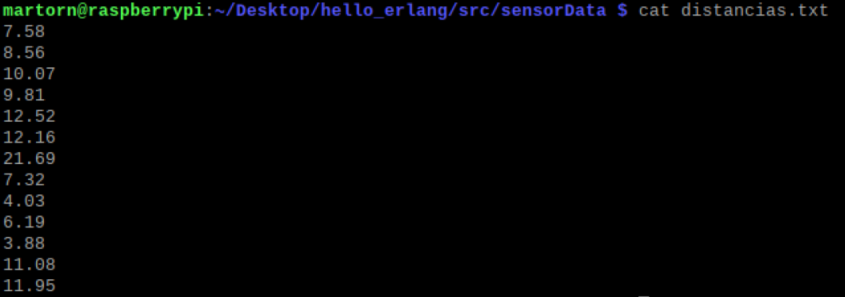
\includegraphics[scale=0.8]{images/salidaUltrasonidoC.png}
\caption[Salida de terminal del código C del sensor HC-SR04]{Visualización de la salida del terminal de la placa R-Pi del archivo creado por el código programado en C que lanza el sensor HC-SR04.}%
\label{fig:salidaUltrasonidoC}
\end{figure}


\section{Pruebas de frecuencia de lectura}

El HMC5983 es un magnetómetro de tres ejes que se comunica a través de una interfaz I2C, por lo que para modificar la frecuencia de lectura del sensor se deben utilizar comandos I2C.

Para cambiar la frecuencia de lectura del HMC5983, se debe configurar el registro de control de configuración (0x00). En este registro, los bits 5-2 controlan la tasa de datos, la cual se puede configurar entre los valores del 0 al 7. La frecuencia de muestreo más alta posible en el caso de este sensor es de 75 Hz por lo que será a la frecuencia a la que con configuraremos para que trabaje en su máximo rendimiento.

Con el comando: 
\begin{lstlisting}[style=terminal]
sudo i2cset -y 1 0x1E 0x00 [valor] 
\end{lstlisting}

Donde valor es el valor de configuración deseado en hexadecimal. Por ejemplo, para configurar una tasa de datos de 75 Hz, el valor se debe establecer en 0x70:

\begin{lstlisting}[style=terminal]
sudo i2cset -y 1 0x1E 0x00 0x70  
\end{lstlisting}


Mediante el comando anterior ya tenemos configurado el sensor para que lea datos en su máxima frecuencia disponible.\\

Al configurar la frecuencia en 75Hz conseguimos que el sensor obtenga una frecuencia de salida de datos de 75 por segundo, esto significa que el sensor proporcionará una nueva medición cada 1/75 segundos o 0.0133 segundos (aproximadamente cada 13 milisegundos), realmente el sensor tiene tres modos de uso; bajo, medio y alto (220 hz) pero para el uso del modo de alta frecuencia es necesario incluir resistencias. Se puede obtener también datos de temperatura del sensor a través de las direcciones 0x31 y 0x32 por si fuera necesario, en este caso no las utilizaremos. Todos estos datos se obtienen del datasheet del sensor.

El siguiente paso es comprobar si esa frecuencia de lectura es posible y nuestro programa C es capaz de leer a una velocidad igual o superior, para plantearnos esta situación debemos observar a qué frecuencia de lectura los datos comienzan a repetirse, en este punto existen dos posibilidades; que la frecuencia de lectura del código C sea superior a la que el sensor lee datos o que el código no sea suficientemente rápido como para leer a la frecuencia máxima del sensor.

A continuación, se realizaron varias pruebas a la frecuencia máxima del sensor modificando el ratio y el tiempo de lectura para observar si los datos comienzan a repetirse o el programa es capaz de almacenar todos los datos obtenidos por el sensor (tablas de los Cuadros \ref{tab:pf005}, \ref{tab:pf01} y \ref{tab:pf008}), durante las cuales se ha movido el sensor de manera aleatoria (movimientos de mano y muñeca) para que este vaya captando diferentes grados de cabeceo.


\begin{table}[htbp]
  \centering
  {\sffamily\small
  \begin{tabular}{|*{10}{r|}}
        \hline
    \multicolumn{10}{c}{\textbf{Prueba de frecuencia 1}: Medidas de ángulo de cabeceo (grados).}\\
    \hline
    35.25 & 35.25 & 35.26 & 35.26 & 35.25 & 45.00 & 45.00 & 44.98 & 44.97 & 44.98\\
    \hline
    44.98 & 44.98 & 35.25 & 35.28 & 35.27 & 35.27 & 35.26 & 35.25 & 35.24 & 35.22 \\
    \hline
    35.22 & 0.02 & 0.02 & 0.02 & 0.02 & 0.02 & 0.02 & 0.02 & 9.98 & 9.98\\
    \hline
    7.85 & 6.07 & 6.60 & 44.91 & 44.91 & 44.93 & 44.94 & 44.94 & 44.94 & 44.95 \\
    \hline
    44.95 & 59.33 & 59.33 & 45.04 & 18.93 & 45.07 & 45.07 & 11.3 & 11.3 & 11.3 \\
    \hline
  \end{tabular}
  } % fin de cambio de font
  \caption[Prueba de frecuencia 1] {50 primeros datos obtenidos del sensor HMC5983 tras realizar la prueba con una frecuencia de lectura de 0.05 segundos durante 5 segundos}\label{tab:pf005}
\end{table}

\begin{table}[htbp]
  \centering
  {\sffamily\small
  \begin{tabular}{|*{10}{r|}}
        \hline
    \multicolumn{10}{c}{\textbf{Prueba de frecuencia 2}: Medidas de ángulo de cabeceo (grados).}\\
    \hline
    0.05 & 0.04 & 6.22 & 8.43 & 8.32 & 10.61 & 10.30 &  35.30 & 35.29 & 12.29\\
    \hline
    15.29 & 33.35 & 35.34 & 35.35 & 44.96 & 44.97 & 46.47 & 46.95 & 48.93 & 48.92 \\
    \hline
    42.78 & 39.91 & 9.73 & 11.87 & 1.08 & 45.05 & 47.05 & 49.06 & 53.08 & 53.11 \\
    \hline
    35.29 & 33.48 & 31.19 & 30.32 & 0.01 & 0.02 & 0.80 & 3.16 & 15.22 & 18.34\\
    \hline
    18.60 & 35.32 & 33.87 & 31.28 & 29.14 & 18.37 & 21.56 & 6.58 & 43.56 & 48.47\\
    \hline
  \end{tabular}
  } % fin de cambio de font
  \caption[Prueba de frecuencia 2]{50 primeros datos obtenidos del sensor HMC5983 tras realizar la prueba con una frecuencia de lectura de 0.08 segundos durante 5 segundos}\label{tab:pf008}
\end{table}

\begin{table}[htbp]
  \centering
  {\sffamily\small
  \begin{tabular}{|*{10}{r|}}
      \hline
    \multicolumn{10}{c}{\textbf{Prueba de frecuencia 3}: Medidas de ángulo de cabeceo (grados).}\\
    \hline
    35.22 & 0.06 & 0.05 & 3.08 & 5.78 & 49.31 & 0.20 & 0.20 & 35.24 & 15.22 \\
    \hline
    17.30 & 35.33 & 31.60 & 31.30 & 35.29 & 45.98 & 55.30 & 58.32 & 40.97 & 44.98\\
    \hline
    44.99 & 41.58 & 0.11 & 0.09 & 3.06 & 5.02 & 25.30 & 35.28 & 39.78 & 35.22\\
    \hline
    33.91 & 31.20 & 35.25 & 34.19 & 29.23 & 35.28 & 39.30 & 44.97 & 46.76 & 44.13\\
    \hline
    41.89 & 35.22 & 37.9 & 35.30 & 11.33 & 8.30 & 2.25 & 1.33 & 6.89 & 7.47\\
    \hline
  \end{tabular}
  } % fin de cambio de font
  \caption[Prueba de frecuencia 3]{50 primeros datos obtenidos del sensor HMC5983 tras realizar la prueba con una frecuencia de lectura de 0.1 segundos durante 5 segundos}\label{tab:pf01}
\end{table}

\clearpage

En la \textbf{prueba de frecuencia 1} se han obtenido 100 datos, de los cuales, los 50 primeros se muestran en la tabla del Cuadro~\ref{tab:pf005}, en ella puede observarse como estos datos se repiten de manera continuada hasta en grupos de 7 elementos, esto denota que el programa está almacenando más datos de los que el sensor puede registrar, es por ello que cuando el programa solicita un dato nuevo este recoge el mismo que el recibido anteriormente.

En la \textbf{prueba de frecuencia 2} se han obtenido 62 datos de los que analizaremos los 50 primeros que se muestran en la tabla del Cuadro~\ref{tab:pf008}, como podemos ver en este caso los datos son diferentes entre sí y varían de forma progresiva sin saltos de ángulo demasiado pronunciados. 

Por último, en la tabla del Cuadro~\ref{tab:pf01} se muestran los 50 datos obtenidos durante la \textbf{prueba de frecuencia 3}, en este caso el ratio de lectura ha sido mucho más lento que en la prueba anterior, al ser un ratio de lectura menor, se han obtenido menos datos pero estos son siempre diferentes entre sí con saltos más significativos que en el caso de la prueba de frecuencia 2. Esto puede ser porque el sensor está leyendo a una frecuencia superior al programa y por tanto se están perdiendo datos.

En conclusión, una frecuencia de lectura óptima sería la utilizada en la prueba de frecuencia 2 (ratio=0.08 segundos) ya que en ella los datos no aparecen tan repetidos como en la prueba de frecuencia 1 y a su vez se obtienen muchos más datos válidos que en la prueba de frecuencia 3.